\documentclass[a4paper,11pt]{article}
%% PREAMBEL %%
%% Pakker %%
\usepackage[english, norsk]{babel}
\usepackage{csquotes}
\usepackage{lipsum}
\usepackage[backend=biber, style=ieee]{biblatex}
\addbibresource{bibliography.bib}
\usepackage[hidelinks]{hyperref}
\usepackage[nottoc]{tocbibind}
\setlength{\emergencystretch}{2em}

\usepackage[margin=25mm]{geometry}
\usepackage{graphicx}
\usepackage{pdfpages}
\usepackage{afterpage}
\newcommand\myemptypage{
    \null
    \thispagestyle{empty}
    \addtocounter{page}{-1}
    \newpage
}

\setlength{\parindent}{0em}
\setlength{\parskip}{1em}

\usepackage{pgfplots}
\pgfplotsset{width=7cm, compat=newest}
\usetikzlibrary{patterns}
\usepackage{bchart}
\renewcommand{\bcfontstyle}{}
\usepackage{pgf-pie}
\usepackage{float}
\usepackage{setspace}
\usepackage{tabularx}
\usepackage{xcolor}
\definecolor{codegreen}{rgb}{0,0.6,0}
\definecolor{codegray}{rgb}{0.5,0.5,0.5}
\definecolor{codepurple}{rgb}{0.68,0,0.12}
\definecolor{backcolour}{rgb}{0.96,0.96,0.96}

\usepackage{listings}
\addto\captionsnorsk{\renewcommand{\lstlistlistingname}{Koder}}
\addto\captionsnorsk{\renewcommand{\lstlistingname}{Kode}}

\lstdefinestyle{mystyle}{
    backgroundcolor=\color{backcolour},
    commentstyle=\color{codegray},
    keywordstyle=\color{codepurple},
    numberstyle=\tiny\color{codegray},
    stringstyle=\color{codegreen},
    basicstyle=\ttfamily\footnotesize,
    breakatwhitespace=false,
    breaklines=true,
    captionpos=b,
    keepspaces=true,
    numbers=left,
    numbersep=5pt,
    showspaces=false,
    showstringspaces=false,
    showtabs=false,
    tabsize=2
}

\lstset{style=mystyle}


%% DOKUMENT START %%
\begin{document}

\pagenumbering{roman} % Sidenummerering for forord og TOC

%% FORSIDE %%
\begin{titlepage}
    \vbox{ }

    \vbox{ }

    \begin{center}
        % Øverste del av siden
        
\includegraphics[width=0.6\textwidth]{img/tekreal}\\[4cm]
        \textsc{\Large IKT218-G 25V - Advanced operating systems}\\[0.7cm]

        % \vbox{ }
        % Tittel
        \noindent\makebox[\linewidth]{\rule{.7\paperwidth}{.6pt}}\\[0.7cm]
        { \huge \bfseries AI Alcatraz operating system}\\[0.25cm]
        \noindent\makebox[\linewidth]{\rule{.7\paperwidth}{.6pt}}\\[0.7cm]
        \large{Spring 2025}\\[1.2cm]
        \vfill
        % Forfatter
        \large
        % \emph{Skrevet av:}\\[1mm]
        Oskar Juell, Alward Munir Jarkin, Kasper Johan Haukland Jacobsen 

        % Nederste del av siden
        {\large \today}
    \end{center}
\end{titlepage}

%% Declaration %%
\include{template/declaration.tex}

%% INNHOLDSFORTEGNELSE %%
\setlength{\parskip}{.5em} % Setter linjeavstander i TOC litt mindre
\cleardoublepage
\tableofcontents
\setlength{\parskip}{1em} % Går tilbake til standard avstand
\newpage

%% SAMMENDRAG & FORORD %%



\pagenumbering{arabic} % Sidenummerering for resten av dokumentet

%% SEKSJONER %%
\section{Introduction to Computer Boot Processes}

The process of booting a computer into a functional os may seem easy, but it is actually a complex sequence of operations that works together behind the scenes. This process has evolved over time and differs from directly on hardware applications and virtual machines.   

\subsection{Power-On Self-Test (POST)}
When a computer is powered on, the first critical operation in the booting process is the Power-On Self-Test (POST). This firmware-based diagnostic tool ensures that the essential hardware components are functioning as they should before attempting to boot into an operating system. The POST verifies the integrity of the BIOS/UEFI, tests the CPU, memory, I/O devices and storage devices. ~\cite{post}.

The POST process communicates its status through beep codes or error messages, providing an essential diagnostic layer before the operating system loads. If the POST process is successful the computer will move on eith the boot process, but if it encounters a major problem an error code is displayed and the user can troubleshoot the issue.    

\subsection{BIOS and UEFI: The System's Foundation}
After a successful POST, control is transferd to either the Basic Input/Output System (BIOS) or its modern successor, the Unified Extensible Firmware Interface (UEFI). While BIOS has served as the firmware interface for a long time, UEFI has largely replaced it in most systems, offering advantages such as support for larger boot drives, faster startup times, and enhanced security features like Secure Boot~\cite{uefi_wiki}.

The firmware's primary responsibility is to identify a boot-able device following the configured boot sequence (solid state drive, hard disk, USB device, network, etc.) and transfer control to its bootloader. UEFI's superiority lies in its ability to understand partition tables and file systems, allowing it to direct access to boot loaders stored as files instead of requiring them to be located in specific physical sectors as it was with the older BIOS~\cite{ms_secureboot}.

\subsection{Bootloaders: Bridging Firmware and Operating Systems}
Bootloaders serve as the critical bridge between firmware and the operating system kernel. Their complexity ranges from simple programs that just load a kernel to sophisticated environments that provide boot menus, hardware configuration options, and multiple OS selection \cite{OSDEV_Bootloader}.

Common bootloaders include:
\begin{itemize}
    \item \textbf{GRUB (Grand Unified Bootloader)} - The default for many Linux distributions, supporting multiple operating systems and kernel options \cite{GRUB}
    \item \textbf{Windows Boot Manager} - Handles the Windows boot process with support for multi-booting and BitLocker encryption \cite{Win_boot}
    \item \textbf{Limine} - A modern, feature-rich bootloader targeting hobby OS development with extensive Multiboot2 support~\cite{limine}
\end{itemize}

The bootloader's essential functions include initializing hardware to a state suitable for the operating system, loading the kernel into memory, and passing control with any required parameters. Modern bootloaders like GRUB2 and Limine are effectively mini-operating systems themselves, with filesystem drivers, configuration files, and modular designs.

\subsection{Memory Layout During Boot}
In traditional x86 architecture, the memory layout during boot follows historical patterns dating back to early PC designs. After the system initializes, the memory starting at address 0x10000 (64KB) is typically where many operating systems load their kernels. This custom started partly because the first 64KB may contain important BIOS data structures ~\cite{kernelboot}.

The traditional memory map includes:
\begin{figure}[H]
    \centering
    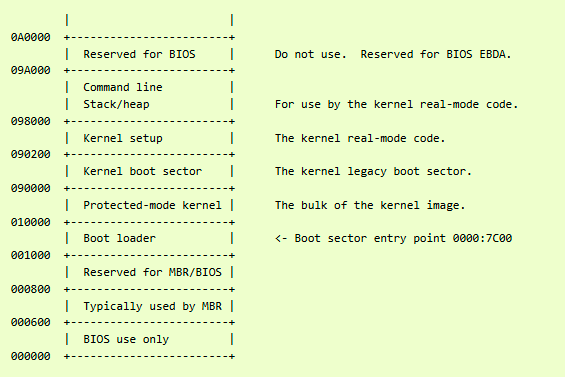
\includegraphics[width=0.9\textwidth]{img/boot_memory.png}
    \caption{Memory map \cite{kernelboot}}
    \label{fig:graph1}
\end{figure}

The choice of 0x10000 as a common kernel loading address provides sufficient space after the boot sector while remaining within the first megabyte of addressable memory in real mode. As the system transitions to protected mode, this memory layout changes significantly as the operating system initializes its own memory management structures.

\subsection{Virtual Machine Boot Process}
The boot process in virtual machines differs fundamentally from the regular hardwere process , although it simulates many of the same steps that is actually done with hardwere booting. Instead of actual firmware, VMs use emulated or paravirtualized BIOS/UEFI implementations provided by a hypervisor. The POST process is normally simulated, focusing on initializing the virtual devices rather than actually testing physical hardware components~\cite{vmboot}.

The key difference lies in the hypervisor's role as an intermediary layer between the virtual machine and the physical hardware by allocating resources and using simulated drivers. This abstraction allows multiple operating systems to share the same physical hardware without conflicts such as running multiple VMs on one hardware machine. The virtualization layer adds flexibility to the boot process while introducing additional complexity in terms of resource management and performance considerations.

\subsection{Evolution of Boot Processes in Modern Systems}
Modern operating systems have evolved their boot processes significantly to meet demands for faster startup times, enhanced security, and support for new hardware technologies. Windows has moved from the simple DOS-based boot process to sophisticated boot managers supporting features like BitLocker, Secure Boot, and Fast Startup (which is a hybrid between hibernation and a full boot)~\cite{ms_secureboot}. Linux systems have evolved from LILO to GRUB2 and systemd-boot, with increased parallelization during initialization to reduce boot times\cite{LILO} \cite{GRUB}.

The introduction of UEFI has been particularly transformative, bringing capabilities such as:
\begin{itemize}
    \item Secure Boot to verify the integrity of boot components
    \item Support for boot drives larger than 2TB
    \item Network booting with greater protocol support
    \item A standardized pre-OS environment with graphics capabilities
\end{itemize}

These advancements reflect the ongoing evolution of boot processes to balance security, performance, and flexibility in increasingly complex computing environments.









\section{Booting and Printing}
In this chapter we implement the first requirements of the task. First we need to boot the operating system, so we have some thing to build the rest on. After this can we implement som simple printing, based on the printf function in C.

\subsection{Multiboot2 Implementation}
First we focused on implementing a proper boot process according to the Multiboot2 specification \cite{Multiboot} \cite{multiboot2}. This included configuring a multiboot header with the correct magic numbers and flags to ensure compatibility with a bootloader \cite{Magic_number}. We configured the Limine bootloader to load our kernel at the correct memory address and with appropriate permissions \cite{limine}. Then asembly code was written in the file \texttt{multiboot2.asm} to manage the transition from bootloader to kernel initialization. This included setting up the stack and invoking the kernel's entry point, written in C.

Additionally, we implemented parsing of the multiboot information structure, allowing the kernel access to system details such as memory maps, module information, and boot device details \cite{multiboot2}. This foundational implementation ensured that our kernel had all necessary context for successful initialization early in the boot process.



\begin{lstlisting}[language=nasm]
section .multiboot
align 8
header_start:
    dd 0xe85250d6                ; magic number
    dd 0                         ; architecture 0 (i386)
    dd header_end - header_start ; header length
    ; ... additional header information ...
header_end:

section .text
global _start
_start:
    mov esp, stack_top  ; Set up stack
    push ebx            ; Pass multiboot info structure
    extern kernel_main
    call kernel_main    ; Call C entry point
\end{lstlisting}

\subsubsection{Key Files for Booting}
\begin{itemize}
    \item \texttt{multiboot2.asm} - This assembly file contains the multiboot header with the required magic values and flags \cite{Magic_number}. It sets up the initial stack, aligns the CPU state, and jumps to the kernel's C entry point. The file also includes sections for early exception handling that might occur before the IDT is set up \cite{multiboot2} \cite{Multiboot}.
    
    \item \texttt{multiboot2.h} - Defines the data structures for parsing the multiboot information provided by the bootloader. This includes structures for memory maps, module information, and bootloader name. The header provides functions to traverse the multiboot tags and extract required information \cite{multiboot2} \cite{Multiboot}.
    
    \item \texttt{kernel.c} - Contains the \texttt{kernel\_main()} function, which is the entry point called from \texttt{multiboot2.asm}. It initializes all subsystems in the correct order (GDT, IDT, memory, keyboard, PIT in the future) and implements the main execution loop of the operating system.
    
    \item \texttt{linker.ld} - The linker script defines the memory layout of the kernel binary, specifying section addresses and alignments required by the Multiboot2 specification. It ensures the multiboot header appears at the beginning of the kernel image \cite{Multiboot}.
\end{itemize}

\subsection{Global Descriptor Table (GDT)}

Next we implemented the Global Descriptor Table (GDT). The GDT defines memory segments and their privilege levels for the CPU. It is used for memory protection in the x86 architecture \cite{osdev_gdt}. In our implementation, we created a structure for the GDT entries in the file \texttt{GDT.h}, where we defined segment descriptors for null, kernel code, and kernel data \cite{osdev_gdt}.

We also wrote an assembly routine in the file \texttt{gdt\_flush.asm}. This routine loads the GDT using the LGDT instruction and updates the segment registers with a far jump, making sure the CPU switches to the new segment layout \cite{osdev_gdt}. This setup is needed for features like paging and user-mode execution and helps make the system more stable and secure.

\begin{lstlisting}[language=c]
typedef struct {
    uint16_t limit_low;    // Lower 16 bits of limit
    uint16_t base_low;     // Lower 16 bits of base
    uint8_t  base_middle;  // Next 8 bits of base
    uint8_t  access;       // Access flags
    uint8_t  granularity;  // Granularity flags + upper 4 bits of limit
    uint8_t  base_high;    // Upper 8 bits of base
} __attribute__((packed)) gdt_entry_t;

typedef struct {
    uint16_t limit;        // The upper 16 bits of all selector limits
    uint32_t base;         // The address of the first gdt_entry_t structure
} __attribute__((packed)) gdt_ptr_t;

// Initialize GDT
void init_gdt();
\end{lstlisting}

\subsubsection{Key Files for GDT Implementation}
\begin{itemize}
    \item \texttt{GDT.h} - Defines the structure of a GDT entry (\texttt{gdt\_entry\_t}) and the GDT pointer (\texttt{gdt\_ptr\_t}). It also declares functions for initializing the GDT and setting up segment descriptors. This header serves as the interface for other parts of the kernel to interact with the GDT subsystem.
    
    \item \texttt{GDT.c} - Implements the GDT initialization logic. It contains the global GDT array, functions to set up segment descriptors with appropriate access flags, and the main initialization function that configures kernel code and data segments. This file translates the abstract concept of memory segmentation into concrete data structures the CPU can use.
    
    \item \texttt{gdt\_flush.asm} - Contains the assembly routine needed to load the GDT into the CPU's GDTR register and update the segment registers. This file bridges the gap between our C code and the CPU's segmentation mechanism, handling the processor-specific instructions that cannot be expressed in C.
\end{itemize}

\subsection{Console Output System}

Next we made a console output system to help with debugging and showing messages on screen. It is written in \texttt{printf.h} and writes characters directly to VGA memory at address \texttt{0xB8000} \cite{VGA}. We added support for format specifiers like \%s for strings, \%d for numbers, and \%c for characters, like the standard C \texttt{printf} function \cite{PrintFIC}.

The system also handles automatic scrolling when the text reaches the bottom of the screen and keeps the cursor in the right place. To control the screen hardware, we used port I/O and the \texttt{outb} function to send values to the VGA ports \cite{OSDev_IOPorts}.
%=============== Dette? \/ \/
This console was very useful during development. It helped us see what the system was doing and made it easier to find and fix problems.
%=============== Dette? ^ ^


\begin{lstlisting}[language=c]
// Write a single character to screen
void putchar(char c) {
    uint16_t* video_memory = (uint16_t*)0xB8000;
    
    if (c == '\n') {
        cursor_y++;
        cursor_x = 0;
    } else {
        // Calculate position and write character with attribute
        const size_t index = cursor_y * VGA_WIDTH + cursor_x;
        video_memory[index] = (attrib << 8) | c;
        cursor_x++;
    }
    
    // Handle screen scrolling and cursor update
    // ...
}

// Simple printf implementation
void printf(const char* format, ...) {
    va_list args;
    va_start(args, format);
    
    for (int i = 0; format[i] != '\0'; i++) {
        if (format[i] == '%') {
            i++;
            // Handle format specifiers
            switch (format[i]) {
                case 's': // String
                    puts(va_arg(args, const char*));
                    break;
                case 'd': // Decimal
                    print_decimal(va_arg(args, int));
                    break;
                // ... other format specifiers ...
            }
        } else {
            putchar(format[i]);
        }
    }
    
    va_end(args);
}
\end{lstlisting}

\subsubsection{Key Files for Console Output}
\begin{itemize}
    \item \texttt{printf.h} - Implements a text output system including formatted printing functions (\texttt{printf}, \texttt{puts}, \texttt{putchar}), cursor control, and screen management. The file contains all necessary code for manipulating the VGA text mode buffer and controlling the hardware cursor through port I/O \cite{VGA} \cite{PrintFIC}.
    
    \item \texttt{stdio.h} - This file is in the \texttt{libc/} folder. It declares the standard input and output functions that are common in C, like \texttt{printf()}. It helps make our code look like C and connects standard C style with our own system \cite{PrintFIC}.
    
\end{itemize}


\subsection{Printing in our OS}

\begin{figure}[H]
    \centering
    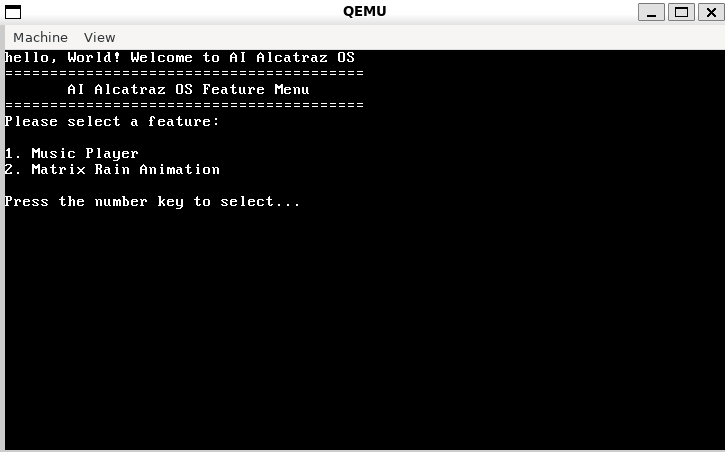
\includegraphics[width=0.9\textwidth]{img/OS_Print.png}
    \caption{Printing out menu}
    \label{fig:graph1}
\end{figure}

As shown in the figure above of our operating system, the printing functionality is used to present a menu used for navigating the functions that will be added later on.  


\section{Interrupts}

In this chapter we explain how interrupts are used in our system. First we set up the IDT, which is needed to handle interrupts. Then we show how to connect the PIC and how we use interrupts to read from the keyboard. At the end, we show how the system handles CPU exceptions to avoid crashes and show helpful error messages.

\subsection{Interrupt Descriptor Table (IDT)}

After setting up the console, we made the Interrupt Descriptor Table (IDT). The IDT lets the CPU react to both hardware and software interrupts, which is important for system control \cite{OSDev_IDT}.

We defined the structure of the IDT in \texttt{IDT.h}, following the x86 format for interrupt gates \cite{OSDev_IDT}. In \texttt{IDT.c}, we wrote functions to fill out the table and load it into the CPU using the LIDT instruction \cite{OSDev_IDT}.

We also made small assembly stubs in \texttt{interrupt.asm} that save the CPU state when an interrupt happens, call the correct C handler, and then restore the state before continuing. To make the system more flexible, we added a way to register different functions for different interrupt numbers. This lets us organize the code better and makes it easier to update or add new handlers \cite{OSDev_Interrupts}.

The purpose of the IDT, is so the system can handle events like keyboard input, exceptions, and system calls. It is a key part of how the system stays responsive and stable.

\begin{lstlisting}[language=c]
typedef struct {
    uint16_t base_low;     // Lower 16 bits of handler address
    uint16_t selector;     // Kernel segment selector
    uint8_t  always0;      // Always zero
    uint8_t  flags;        // Flags (type and attributes)
    uint16_t base_high;    // Upper 16 bits of handler address
} __attribute__((packed)) idt_entry_t;

void init_idt();
void register_interrupt_handler(uint8_t num, void (*handler)(registers_t*));
\end{lstlisting}

\subsubsection{Key Files for IDT Implementation}
\begin{itemize}
    \item \texttt{IDT.h} - Defines the structure of an IDT entry (\texttt{idt\_entry\_t}) and the IDT pointer (\texttt{idt\_ptr\_t}). It also declares functions for initializing the IDT, registering interrupt handlers, and configuring the Programmable Interrupt Controller. This header serves as the interface for the interrupt subsystem.
    
    \item \texttt{IDT.c} - Implements the IDT setup and management. It contains the global IDT array, functions to set up interrupt gates with appropriate flags, and PIC initialization code. This file handles the configuration of interrupt controllers and maintains the table of interrupt handlers.
    
    \item \texttt{interrupt.asm} - Contains assembly language interrupt service routines (ISRs) that respond to CPU exceptions and hardware interrupts. These routines save the CPU state, call the appropriate C handler function, and restore the state before returning. This file handles the low-level processor-specific aspects of interrupt handling \cite{OSDev_Interrupts}.
\end{itemize}

\subsection{Programmable Interrupt Controller (PIC)}

To handle hardware interrupts properly, we set up the Programmable Interrupt Controller (PIC). The PIC is responsible for sending signals from hardware devices to the CPU. We remapped the default IRQs to avoid overlapping with CPU exceptions by moving them to interrupt numbers 32–47 \cite{OSDev_PIC} \cite{PrintFIC}.

After an interrupt is handled, we send an End of Interrupt (EOI) signal to the PIC. This tells the controller it is ready to handle the next interrupt. We also made it possible to enable or disable specific IRQ lines by masking or unmasking them. This gives us more control over which devices can send interrupts \cite{OSDev_PIC} \cite{OSDev_Interrupts}.

By using interrupts instead of constantly checking devices, the CPU can do other work and respond only when needed. This makes the system faster and more efficient. The PIC is an important part of the system and helps connect hardware with the rest of the operating system.


\subsubsection{Key Files for PIC Management}
\begin{itemize}
    \item \texttt{IDT.c} - While not a dedicated PIC file, this contains the PIC initialization code (\texttt{pic\_remap}) and helper functions for sending commands to the PIC. It handles the remapping of IRQs to avoid conflicts with CPU exceptions and provides functions to mask/unmask specific interrupt lines \cite{OSDev_PIC} \cite{OSDev_Interrupts}.
\end{itemize}

\subsection{Keyboard Handler}

To show how our interrupt system works in practice, we added a keyboard handler that uses IRQ1. We set up IRQ1 and connected it to our handler function using the IDT \cite{OSDev_Keyboard} \cite{OSDev_Interrupts}.

When a key is pressed or released, the scan code is read from I/O port \texttt{0x60}, which is the keyboard’s data port. We used a 64-byte circular buffer to store the scan codes, so fast key presses would not be lost if the system was busy.

The scan codes are converted to ASCII characters using a lookup table that matches standard keyboard layouts \cite{ASCII}. We also made it possible for programs to register their own callback functions to react to certain keys.

This part of the system shows how hardware events, like key presses, can be handled using interrupts to create interactive features. It explains how the system responds to input in real time by combining interrupt handling, keyboard decoding, and modular design to make a responsive user interface.


\subsubsection{Key Files for Keyboard Handling}
\begin{itemize}
    \item \texttt{keyboard.h} - Declares keyboard-related structures and functions, including the keyboard buffer interface, scan code to ASCII mapping, and callback registration functions. This header defines how other parts of the kernel can interact with the keyboard subsystem \cite{ASCII} \cite{OSDev_Keyboard}.
    
    \item \texttt{keyboard.c} - Implements the keyboard interrupt handler and input processing logic. It contains the keyboard buffer implementation, scan code translation functions, and the IRQ1 handler that reads from the keyboard controller. This file bridges the hardware keyboard interface with the software input processing system \cite{OSDev_Keyboard} \cite{OSDev_Interrupts}.
\end{itemize}

\subsection{Exception Handling}

To support stability and error reporting, the system includes handlers for several CPU exceptions. For example, the divide-by-zero exception (INT 0) helps detect illegal math operations and shows an error message instead of letting the system crash \cite{OSDev_Exceptions}.

We also included a breakpoint exception (INT 3) that is useful for debugging. It allows the developer to stop the system at specific points and check the state of the CPU. The general protection fault (INT 13) handles serious errors, like when user programs try to access restricted memory or use special CPU instructions \cite{OSDev_Exceptions}.

Each exception handler prints out information such as the instruction address and register values at the time of the error. This helps during debugging and makes it easier to understand what went wrong.

Handling exceptions like this is an important part. It helps prevent crashes and keeps the system running even when something goes wrong.


\subsubsection{Key Files for Exception Handling}
\begin{itemize}
    \item \texttt{IDT.c} - Contains the implementations of exception handlers for various CPU exceptions, such as divide by zero, breakpoint, and general protection fault. These handler functions display diagnostic information and manage the system's response to exceptional conditions \cite{OSDev_Exceptions}.
    
    \item \texttt{interrupt.asm} - Provides the low-level exception entry points that save the CPU state and call the appropriate C handlers defined in IDT.c. This file contains assembly code that handles the processor-specific aspects of exception processing.
\end{itemize}


\subsection{Interups in our OS}

\begin{figure}[H]
    \centering
    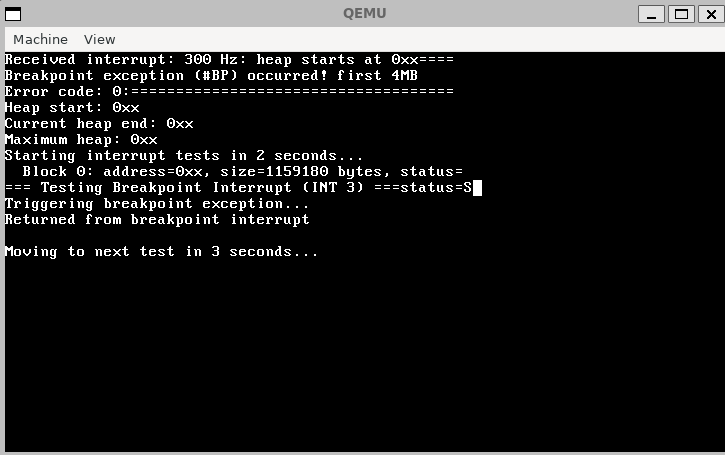
\includegraphics[width=0.9\textwidth]{img/interupt_test_1.png}
    \caption{Testing interrupts}
    \label{fig:graph1}
\end{figure}

\begin{figure}[H]
    \centering
    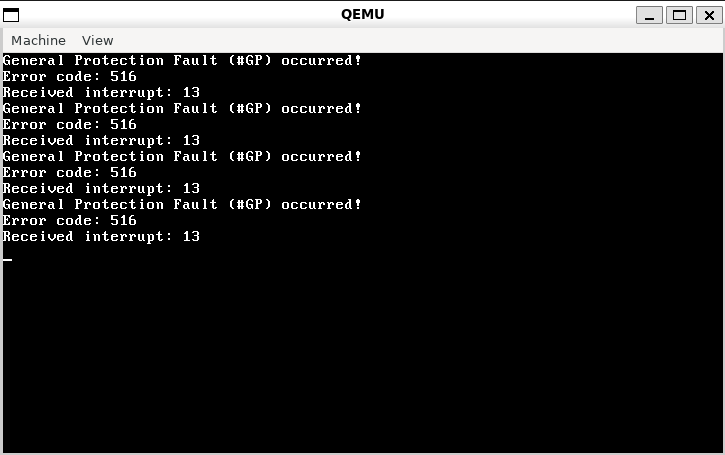
\includegraphics[width=0.9\textwidth]{img/interupt_test_2.png}
    \caption{Testing interupts}
    \label{fig:graph1}
\end{figure}

\begin{figure}[H]
    \centering
    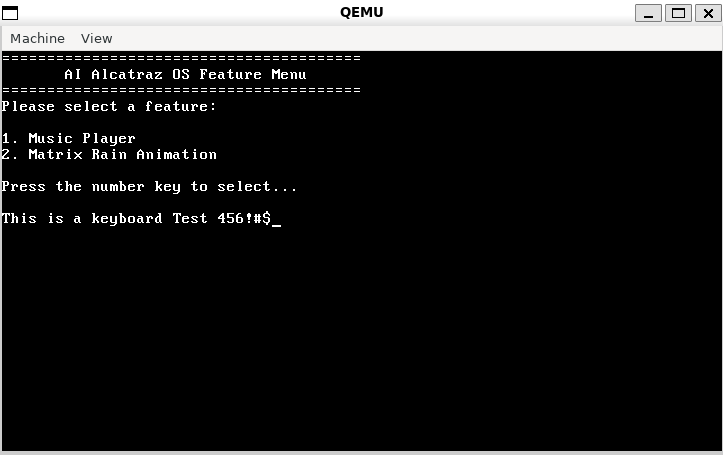
\includegraphics[width=0.9\textwidth]{img/keyboard.png}
    \caption{Testing Keyboard}
    \label{fig:graph1}
\end{figure}

\section{Memory and PIT}

In this chapter we look at two important systems: memory management and the timer. First we add support for dynamic memory by making a heap and basic versions of \texttt{malloc()} and \texttt{free()}. Then we add paging, which lets the CPU use virtual memory and helps protect the system from memory errors. After that, we explain how we use the Programmable Interval Timer (PIT) to keep track of time and run code at the right moment. 

\subsection{Memory Management System}

To support dynamic memory in our kernel, we implemented a simple memory management system. It starts by setting up a heap, which is a block of memory used for dynamic allocations \cite{OSDev_Heap}.

We wrote basic versions of \texttt{malloc()} and \texttt{free()} to let the system allocate and free memory while it is running \cite{GNU_malloc}. These functions work directly with physical memory. When a smaller block is requested, the allocator can split a larger block into two parts to reduce wasted space \cite{MemoryAllocation}. We also used a first-fit algorithm to find the first free block that is large enough \cite{FirstFit}. This to make a balance between performance and memory fragmentation.

The heap can grow up to 16MB if more memory is needed. This means the system is not limited to a fixed amount of memory and can adjust as more programs or features are added. It helps the system work better under different conditions, such as when running larger programs or many tasks at once. Both the kernel and other parts of the OS can safely request memory through this system, making it more reliable and easier to scale \cite{OSDev_Heap}.

Having this memory system in place helps us build other parts of the OS. It lets us manage memory in a controlled way and makes it easier to add new features later.


\subsubsection{Key Files for Memory Management}
\begin{itemize}
    \item \texttt{memory.h} - Declares memory management functions, constants, and data structures, including the memory block header used by the allocator. It defines interfaces for memory allocation, deallocation, and manipulation.
    
    \item \texttt{memory.c} - Implements the heap initialization, memory allocation (\texttt{malloc}), and deallocation (\texttt{free}) functions. It contains the first-fit allocation algorithm and memory block management logic. This file also includes physical memory management for the kernel's needs \cite{GNU_malloc} \cite{FirstFit} \cite{MemoryAllocation}.
    
    \item \texttt{string.h} - Located in the \texttt{libc/} directory, this file declares memory manipulation functions like \texttt{memcpy}, \texttt{memset}, and \texttt{memcmp} that operate on arbitrary memory regions \cite{OSDev_String}.
\end{itemize}

\subsection{Paging Implementation}

To add memory protection and support virtual memory, we made a paging system. Paging lets the CPU use virtual addresses and map them to physical memory. This adds flexibility and helps stop programs from accessing memory they should not \cite{OSDev_Paging}.

We started by identity-mapping the first 4MB of memory. This means that virtual and physical addresses were the same, which made it easier to get the system running in the beginning. We also made functions that let the kernel allocate, free, and map physical memory pages \cite{OSDev_Paging}.

To turn on paging, we set a special bit in the CR0 control register. After that, the CPU started using the page directory and page tables to translate addresses. This also let us mark certain memory areas as read-only or inaccessible, which improves safety and helps avoid bugs \cite{OSDev_Paging}.

Having paging in place is important for more advanced memory features. It lets the system support things like process isolation, memory-mapped I/O, and better memory sharing through methods like copy-on-write. 



\subsubsection{Key Files for Paging}
\begin{itemize}
    \item \texttt{memory.h} - Includes declarations for paging-related functions and structures, such as page directory and page table entry formats. It defines the interface for page allocation, mapping, and permission management \cite{OSDev_Paging}.
    
    \item \texttt{memory.c} - Contains the paging implementation, including functions to initialize paging, allocate and map pages, and modify page attributes. This file handles the creation and management of page directories and tables, as well as the low-level code to enable paging in the processor \cite{OSDev_Paging}.
\end{itemize}

\subsection{Programmable Interval Timer (PIT)}

To keep track of time in the system, we added support for the Programmable Interval Timer (PIT). We used channel 0 in rate generator mode, which sends out regular signals based on a set divisor \cite{OSDev_PIT}. This gives us control over how often the timer fires and lets us balance between precision and performance.

We made a tick counter that goes up every time the timer sends an interrupt. This helps us know how long the system has been running. It is also used for features like delays and scheduling \cite{OSDev_PIT}.

We made two delay functions: \texttt{sleep\_busy()} and \texttt{sleep\_interrupt()}. The first one waits by using the CPU in a loop and is good for short waits. The second one uses interrupts and is better for longer waits, since it lets the CPU do other work during the wait \cite{OSDev_PIT}.

The PIT is like the system's clock. It helps us run things at the right time, handle delays, and will be important later if we need to add support for example multitasking.


\subsubsection{Key Files for PIT Implementation}
\begin{itemize}
    \item \texttt{pit.h} - Declares PIT-related constants (like the base frequency of 1.193182 MHz) and functions for timer initialization, configuration, and delay operations. This header defines the timing interface available to other parts of the kernel \cite{OSDev_PIT}.
    
    \item \texttt{pit.c} - Implements PIT initialization, configuration, and timing functions. It contains the IRQ0 handler that processes timer interrupts and increments the system tick counter. This file also implements both busy-wait and interrupt-based sleep functions for different delay requirements \cite{OSDev_PIT}.
\end{itemize}


\subsection{Memory and PIT}


\begin{figure}[H]
    \centering
    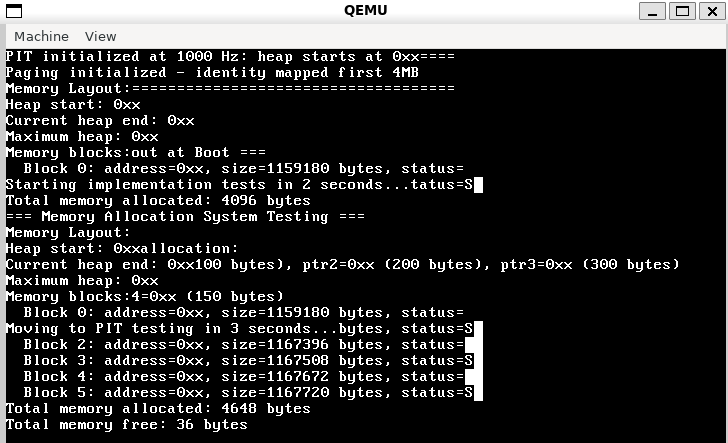
\includegraphics[width=0.9\textwidth]{img/meomory.png}
    \caption{Memory}
    \label{fig:graph1}
\end{figure}

\begin{figure}[H]
    \centering
    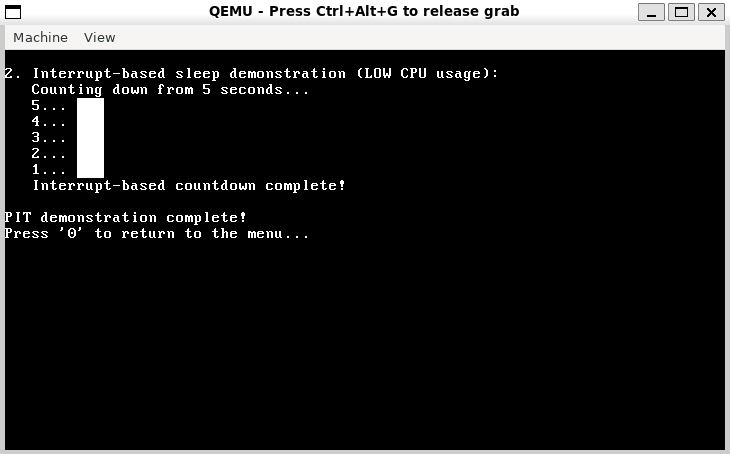
\includegraphics[width=0.9\textwidth]{img/pit_demo_1.png}
    \caption{Pit demo}
    \label{fig:graph1}
\end{figure}

\begin{figure}[H]
    \centering
    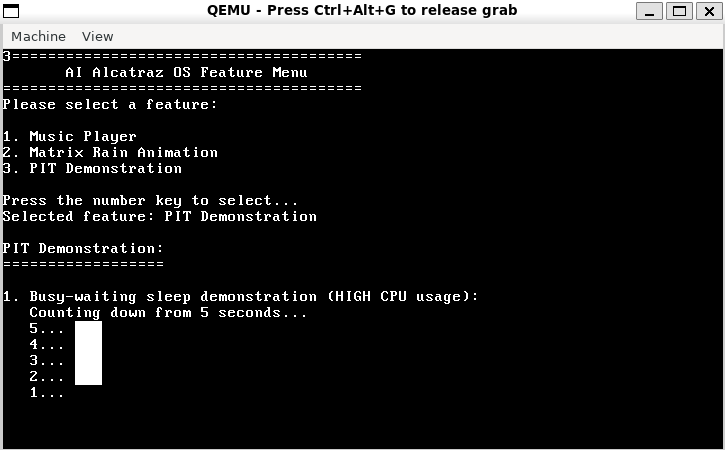
\includegraphics[width=0.9\textwidth]{img/pit_demo_2.png}
    \caption{Pit demo}
    \label{fig:graph1}
\end{figure}


Did some modification to the OS to show the memory and pit functions

\section{Music Player}

In this chapter we describe how we made a simple music player using the PC speaker. This feature helps show how we can use the timer and hardware ports in our system to play a sound.

We started by writing a file called \texttt{frequencies.h}, where each musical note is linked to its frequency in hertz \cite{Note_Frequencies}. In \texttt{song.c}, we made a function that plays songs by looping through a list of notes and playing each one for a short time \cite{OSDev_PC_Speaker}. We used the PIT to time the notes so the rhythm and tempo would be correct \cite{OSDev_PIT}.

To make sound, we programmed the PIT to send out square wave signals at the note's frequency. Then we sent control values to I/O ports \texttt{0x61} and \texttt{0x43} to turn the PC speaker on and off. The speaker only plays while a note is active, so the output sounds clean \cite{OSDev_PC_Speaker} \cite{OSDev_PIT}.

This music player shows how different parts of the system can work together: timing, port I/O, and file structure. 

\subsection{Design and Implementation}

The music player is built using a list of notes where each entry has a pitch and a duration \cite{Note_Frequencies}. This makes it easy to define a full melody as a simple array in the code.

During playback, the system keeps track of which note is currently playing using an index. It then plays each note in order, using the PIT to make sure the note lasts the right amount of time \cite{OSDev_PIT}. Short notes are played using busy-waiting, and longer notes use timer interrupts so the CPU doesn't waste time.

To make the sound, we program the PIT to match the note's frequency and turn the PC speaker on and off using hardware ports \cite{OSDev_PC_Speaker, OSDev_PIT}. This setup combines timing and hardware control.



\begin{lstlisting}[language=c]
void speaker_play_tone(uint32_t frequency) {
    uint32_t divisor = 1193180 / frequency;
    
    // Set PIT channel 2 for speaker frequency
    outb(0x43, 0xB6);
    outb(0x42, divisor & 0xFF);
    outb(0x42, (divisor >> 8) & 0xFF);
    
    // Turn speaker on
    uint8_t tmp = inb(0x61);
    outb(0x61, tmp | 3);
}

void speaker_stop_tone() {
    // Turn speaker off
    uint8_t tmp = inb(0x61);
    outb(0x61, tmp & 0xFC);
}

void play_note(note_t note) {
    if (note.frequency > 0) {
        speaker_play_tone(note.frequency);
        sleep_interrupt(note.duration);
        speaker_stop_tone();
    } else {
        // Silence (rest)
        sleep_interrupt(note.duration);
    }
}
\end{lstlisting}

\subsubsection{Key Files for Music Player}
\begin{itemize}
    \item \texttt{song.h} - Declares music player functions and song data structures. It defines the interface for playing notes and song sequences. This header also includes function prototypes for PC speaker control \cite{OSDev_PC_Speaker}.
    
    \item \texttt{song.c} - Implements the music player functionality, including PC speaker control through port manipulation and song playback logic. It contains functions to play individual notes and complete melodies, managing timing between notes using the PIT subsystem \cite{OSDev_PIT} \cite{OSDev_PC_Speaker}.
    
    \item \texttt{frequencies.h} - Defines constants for musical note frequencies, mapping note names (like A4, C5) to their corresponding frequency values in Hertz. This file provides a musical abstraction layer over the raw frequency values used by the speaker \cite{Note_Frequencies}.
\end{itemize}


\subsection{User Interaction}

Users can start the music player using a simple menu that runs inside the main loop of the kernel. After the system boots, the menu waits for user input, which is handled by our interrupt-based keyboard system \cite{OSDev_Keyboard}. The user can press a specific key to start the music player.

When the music player is selected, the system begins playing a fixed melody right away. This is done without any graphical interface, showing that even a basic menu in text mode can control real system functions. It also demonstrates how timing from the PIT and hardware control through I/O ports can be triggered by keyboard input \cite{OSDev_PC_Speaker} \cite{OSDev_PIT}.

This setup helps show how different parts of the OS—keyboard input, interrupts, timing, and speaker output can work together to create a responsive user experience. Even though the system is minimal, it can still interact with the user in a "meaningful" way.


\subsection{Music player in our OS}

\begin{figure}[H]
    \centering
    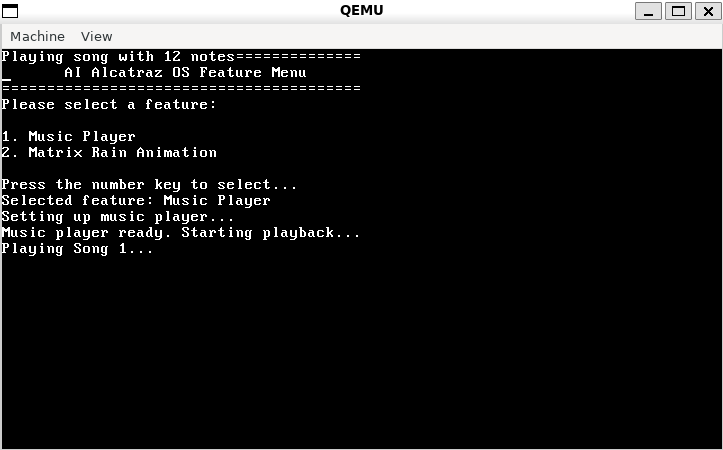
\includegraphics[width=0.9\textwidth]{img/musicplayer.png}
    \caption{Music player}
    \label{fig:graph1}
\end{figure}

Since PDF does not support audio this the our demonstration of the music player implementation 



\section{Matrix Rain Animation}
In this chapter we describe how we built a Matrix-style animation to show what our system can do with simple graphics and timing. The animation is made in text mode using VGA memory and runs directly on our kernel. It helps us test and demonstrate how different low-level parts of the OS like video output, timing, memory management, and random number generation can work together to make a smooth and interesting visual effect.

\subsection{Concept and Design}

We chose to make a matrix rain with graphics in text mode. We made a Matrix-style rain animation based on the digital rain from the movie The Matrix \cite{matrixRainFilm} \cite{matrixRainKode}. It shows how we can make real-time visual effects by writing directly to VGA memory \cite{VGA}.

The animation makes falling columns of random characters that move down the screen like green code rain. We use video memory at \texttt{0xB8000} to draw both characters and their colors \cite{VGA}. This lets us make glowing and fading effects by changing how bright each character is.

To make the rain look more natural, we added random values for where each column starts, how fast it moves, and what characters it shows. Each column behaves independently, and the speed and characters are different each time. This randomness avoids patterns and makes the animation feel more dynamic and alive, like real flowing rain.

For timing, we used the PIT to update the screen at a steady rate \cite{OSDev_PIT}. The PIT sends regular interrupts that we use to trigger screen updates. By adjusting the frequency, we control how fast the characters fall. This makes the animation smooth while keeping CPU usage low, since the updates happen only when needed.


\subsubsection{Key Files for Matrix Animation}
\begin{itemize}
    \item \texttt{matrix.h} - Declares Matrix animation functions and data structures, defining the interface for initializing, updating, and rendering the animation. This header provides functions to start and stop the animation effect \cite{matrixRainFilm} \cite{matrixRainKode}.
    
    \item \texttt{matrix.c} - Implements the Matrix rain animation, including character generation, position tracking, and rendering to the VGA text buffer. It contains the animation loop that updates character positions and attributes for each frame, creating the falling code effect\cite{matrixRainFilm} \cite{matrixRainKode} \cite{VGA}.
\end{itemize}

\subsection{Implementation Details}

The Matrix animation uses our console output system to write directly to VGA memory. Both characters and their color attributes are changed in real time to create the falling code effect with glowing and fading trails. Each column has its own data structure that keeps track of where it is on the screen and what character it is showing \cite{VGA}.

For each frame of the animation, the logic moves the columns one step down, draws a new bright character at the top, and dims the characters below to make it look like a trail. This is all done by writing directly to the VGA memory at \texttt{0xB8000}, using custom color values to match the green-on-black style \cite{VGA}.

The animation timing is controlled by the PIT. It sends interrupts at fixed intervals so the screen updates happen evenly \cite{OSDev_PIT}. When we need temporary memory to manage column data or generate random values, we use the kernel’s memory functions like \texttt{malloc()} \cite{GNU_malloc}.

This project shows how key OS features like video output, timer interrupts, memory allocation, and random number generation can work together. Even with only text mode graphics, we were able to create an interactive and nice-looking animation by combining low-level tools in a creative way.



\begin{lstlisting}[language=c]
void matrix_frame() {
    if (!matrix_running) return;
    
    // Update each drop
    for (int i = 0; i < MAX_DROPS; i++) {
        // Update wait counter
        if (drops[i].wait < drops[i].speed) {
            drops[i].wait++;
            continue;
        }
        drops[i].wait = 0;
        
        // Fade old position and move drop down
        if (drops[i].y >= 0 && drops[i].y < VGA_HEIGHT) {
            // Fade out the character
            uint16_t* vga = (uint16_t*)VGA_MEMORY;
            int pos = drops[i].y * VGA_WIDTH + drops[i].x;
            uint8_t current_attr = (vga[pos] >> 8) & 0xFF;
            
            // Reduce intensity (green value)
            if (current_attr > 0) {
                uint8_t new_attr = current_attr - 1;
                vga[pos] = (new_attr << 8) | (vga[pos] & 0xFF);
            }
        }
        
        drops[i].y++;
        drops[i].character = CHARSET[rand() % CHARSET_LEN];
        
        // Draw at new position if on screen
        if (drops[i].y >= 0 && drops[i].y < VGA_HEIGHT) {
            // Bright green for head of stream
            // ...
        }
        
        // Reset if drop has moved completely off screen
        // ...
    }
    
    // Wait for next frame
    sleep_interrupt(50);  // 20 FPS
}
\end{lstlisting}


\subsection{Matrix rain in out OS}

\begin{figure}[H]
    \centering
    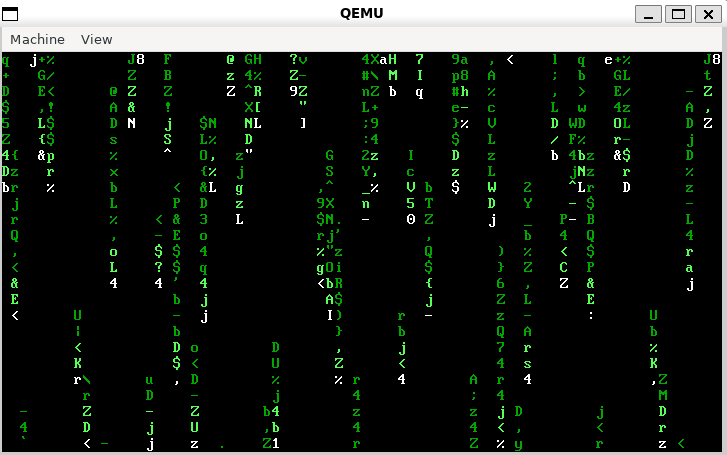
\includegraphics[width=0.9\textwidth]{img/matrix.png}
    \caption{Matrix animation}
    \label{fig:graph1}
\end{figure}


\section{Conclusion}

The development of AI Alcatraz has provided invaluable insight into the internal workings of operating systems. By implementing core components from scratch, we gained hands-on experience with low-level hardware interaction and system design—insight rarely accessible when working solely with high-level abstractions.

One of the key takeaways was the importance of layered system architecture. Each subsystem built upon lower-level mechanisms while abstracting away complexity for higher levels, fostering modularity and enabling us to manage growing complexity without cross-component instability. This principle was essential for maintaining consistency and reliability across our implementation.

Hardware abstraction and direct device control proved to be some of the most challenging aspects. From configuring the PIT to handling I/O ports and implementing the keyboard driver, we developed a deep appreciation for the intricacies of timing and control in real-time systems. Similarly, memory management—including GDT setup, paging, and dynamic heap allocation—formed a stable foundation for the entire kernel, reinforcing the critical role of memory protection in system stability.

The interrupt system, including exception handling, IRQ management, and our custom keyboard handler, was central to achieving responsiveness. These components allowed us to react to hardware events, synchronize execution, and ensure that time-sensitive operations could run efficiently. Moreover, the diagnostic infrastructure—particularly the custom printf and console output systems—proved instrumental in debugging and understanding internal states during development.

Beyond functionality, features such as the music player and Matrix animation demonstrated the expressive potential of low-level operating system design. These modules brought together multiple subsystems—timing, input, memory, and graphics—and highlighted the creative and practical capabilities of a handcrafted OS environment.

This project lays a strong foundation for future exploration in systems programming. The lessons learned through building an OS from the ground up—layered abstraction, hardware interfacing, interrupt-driven design, and real-time control—equip us with valuable tools and perspectives. These insights will remain applicable even as we move toward higher-level technologies, helping us understand what lies beneath the abstraction layers of modern computing systems.

%% BIBLIOGRAFI %%
\printbibliography[heading=bibintoc]
\newpage

%% VEDLEGG %%

%% DOKUMENT SLUTT %%
\end{document}